% Copyright 2022 the authors

% To-Do list:
% -----------
% - What are our GOALS!!?
%   -- one option: this formulation can express all equivariant differential operators discretized to a cubical d-torus. 
%   -- another option: can we produce a characterization of all equivariant functions (maybe based on invariants or these filters) that don't require the use of non-linearities.
%   -- another option: emulate cosmological simulations.
% - change N to N^3 in the appropriate locations; already done??
% - Understand what functions can and cannot be expressed on this model 
% - Extend it to non-linear maps (eg, by multiplications and contractions)
% - Should we be representing images in fourier space? Ask Leslie!
% - Understand the literature
%   -- Discretized vector calculus and differential geometry.
%   -- Group-equivariant CNNs; what's been done?
%   -- Understand how this formulation compares with steerable CNNs
%   -- What is known about what functions CNNs can represent? all linear translation equivariant functions can be written as convvolutions if the filters are as large as the image (simple observation)
% what about non-linear? is there a polynomial basis here? 
%  -- Define "local" functions, is there a characterization of functions that can be written as convolutions with small filters?

% -- if the size of the filter is large enough, are we universal???? or can we express all polynomial functions? is there a version of Stone-Weierstrass for this?
% --- add the identity and levi civita in the possible output tensors
% --- define reordering of the indices
% --- we don't need to be in the torus and we don't need to be square (or cubical)
% --- generalize convolution to rectangular non-toroidal images


%-- is it the same to do convolutions + products + convolutions + products 

%-- a counting argument may tell us that all the linear functions that are equivariant  (Molien's formula)

%-- BEN: compute Molien's formula for this (translations semidirect D_4) action
% 1/|G|\sum_{g\in G} det(I-\phi(g)t)^{-1}

\documentclass{article}
\usepackage[utf8]{inputenc}
\usepackage[letterpaper]{geometry} % because Overleaf is weird.
\PassOptionsToPackage{hyphens}{url}
\usepackage[hidelinks]{hyperref}
\usepackage{graphicx}
\usepackage{amsfonts}
\usepackage{amsmath}
\usepackage{amsthm}

% theorem, definition and so on
\theoremstyle{plain}
\newtheorem{definition}{Definition}
\newtheorem{conjecture}{Conjecture}
\newtheorem{theorem}{Theorem}

% text macros
\newcommand{\sectionname}{Section}
\newcommand{\secref}[1]{\sectionname~\ref{#1}}

% typesetting adjustments
\makeatletter
\renewcommand\section{\@startsection {section}{1}{\z@}%
  {-3.25ex \@plus -1ex \@minus -.2ex}%
  {1.5ex \@plus .2ex}%
  {\raggedright\normalfont\large\bfseries}}
\makeatother
\setlength{\textwidth}{5.00in}
\setlength{\oddsidemargin}{3.25in}
\addtolength{\oddsidemargin}{-0.5\textwidth}
\setlength{\textheight}{9.40in}
\setlength{\topmargin}{-0.50in}
\setlength{\footskip}{0.25in}
\pagestyle{myheadings}
\markboth{foo}{Hogg, Blum-Smith, \& Villar /Geometric filters for geometric images}
\newcommand{\figurerule}{\rule[1ex]{\textwidth}{0.2pt}}
\linespread{1.08}
\frenchspacing\sloppy\sloppypar\raggedbottom

\title{\bfseries%
Equivariant convolution-based functions
on tensor fields}
\author{David W. Hogg, Ben Blum-Smith, and Soledad Villar}
\date{}

\begin{document}

\maketitle\thispagestyle{empty}

\paragraph{Abstract:} We provide a construction for general equivariant convolution-based functions of images or lattices
containing scalars, vectors, and tensors. The formulation, inspired by Einstein summation notation, does not use point-wise activation functions, but it can universally approximate all analytic equivariant functions with respect to discrete rotations of the image. CHECK WITH BEN

\section{Introduction}

Contemporary physics teems with data sets that are images or lattices or grids of geometric objects.
Rectangular images or lattices of density (a scalar field), temperature (also a scalar field), velocity (a vector field), magnetic field (a pseudo-vector field), and polarization (a 2-tensor field) are regularly taken with detectors or made in simulations.
That is, physics has lots of data that consists of geometric objects on regular grids.
These objects (scalars, vectors, pseudo-vectors, and tensors, for example) are \emph{geometric} in the sense that they are defined by their transformation properties under rotation and reflection.
For example, scalars are defined to be quantities in $\mathbb R$ that are invariant with respect to all rotations and reflections; vectors are defined (in $d$-dimensional space) to be quantities in $\mathbb R^d$ that transform under rotation or reflection by multiplication by the orthogonal $d\times d$ matrix representing the rotation or reflection; and so on.

For one concrete example, cosmological n-body simulations comprise the most computationally expensive part of most contemporary cosmological projects, missions, and experiments (CITE THINGS).
For this reason, accurate, fast emulators might be of enormous economic and scientific value.
There are now quite a few successful projects implementing such emulators (CITE THINGS).
Importantly, the initial conditions for these simulations are tiny displacements (vectors) and velocities (vectors) relative to a cubical lattice on a 3-torus.
That is, the initial conditions can be described as a 3-dimensional image of vectors on a regular grid.
For another concrete example, astronomical imaging data taken of the interstellar medium can be represented as rectangular lattices of measurements of temperature (scalar), optical depth (scalar), and induced polarization of starlight (a 2-tensor).
Here the data can be described as a 2-dimensional image of scalars and tensors on a regular grid.

The application of machine-learning techniques to these problems can be dangerous:
Machine-learning models have enormous freedom; the laws of physics are constrained to obey a large set of extremely strict symmetries, including rotation, reflection, translation, permutation, and boost equivariances, plus constraints such as units and dimensions symmetry, unitarity, and myriad conservation laws.
If we want to operate safely on these problems, we want these symmetries built in from the start, and exactly.

HOGG: Differences between continuous and discrete symmetries.

HOGG: Summarize here how we are going to proceed, in human language.


\section{Geometric convolutions}\label{sec:convolution}

We consider the orthogonal group $O(d)$ and $g\in O(d)$. For our purposes $d$ will be 2 or 3, but everything generalizes.  
We consider an image $A$ in a $d$-torus with $N$ equally spaced pixels in each dimension ($N^d$ pixels total). Each pixel can contain tensors and pseudotensors (of which scalars, pseudoscalars, vectors, and pseudovectors are particular cases) that we define below.
Similarly, each linear geometric convolution operator $C$ will be a pixelized cubical image patch with $M$ pixels (with $M$ odd) in each dimension ($M^d$ pixels total) with a tensor or pseudotensor in each pixel, which acts as a linear pixel weight.

For some of the expressions below we will use Ricci and Levi-Civita summation notation (or Einstein summation notation).
In this notation, tensor products are written in component form, and repeated indices are summed over.
In this notation, the product of two 2-tensors (represented as two $d\times d$ matrices $A$ and $B$) is written as
\begin{equation}
    [A\, B]_{i,j} = [A]_{i,k}\,[B]_{k,j} ~,
\end{equation}
where $[A]_{i,k}$ (for example) is the $i,k$ element of matrix $A$, the repeated index $k$ is implicitly summed over the integers from 1 to $d$.
This notation works for tensor expressions of any order, provided that every index appears either exactly once (so it isn't summed over; in the above expression $i, j$ appear exactly once) or exactly twice (so it is summed over; in the above expression $k$ appears exactly twice). 

\begin{definition}[vectors, scalars, and $k$-tensors] \label{def.tensors}
We say that $v\in \mathbb R^d$ is a vector (or 1-tensor) if $O(d)$ acts on $v$ via the canonical action. Namely, for any $g\in O(d)$ we have $g\cdot v = M(g)\, v$ where $M(g)\in \mathbb R^{d\times d}$ is the the matrix representation of $g$. We say that $a\in \mathbb R$ is a scalar (or 0-tensor) if $O(d)$ acts trivially on $a$. Namely $g\cdot a = a$.
We say that $T\in (\mathbb R^d)^{\otimes k}$ is a $k$-tensor if $O(d)$ acts on $T$ as follows:
$O(d)$ acts on a rank-1 $k$-tensor by $g\cdot (v_{1}\otimes\ldots \otimes v_k) = (g\cdot v_1)\otimes \ldots \otimes (g\cdot v_k)$ and it acts on higher rank tensors by linearly extending the actions to linear combinations of such rank-1 $k$-tensors.
\end{definition}

One consequence of the above definitions is that 
$T\in (\mathbb R^d)^{\otimes k}$ is a $k$-tensor iff (in summation notation)
$[g\cdot T]_{i_1,\ldots, i_k} = [T]_{j_1,\ldots,j_k}\,[M(g)]_{i_1,j_1}\cdots[M(g)]_{i_k,j_k}$ for all $g\in O(d)$, where $[T]_{i_1, \ldots ,i_k} \in \mathbb R$ is a component of $T$, $[M(g)]_{i,j}\in\mathbb R$ is the $i,j$ element of the matrix representation of $g$, and all the $i_m$ and $j_m$ are indices in the range $1,\ldots,d$.
For example, a 2-tensor is defined by its transformation property
$[g\cdot T]_{i,j} = [T]_{k,\ell}\,[M(g)]_{k,i}\,[M(g)]_{\ell,j}$,
which, in normal matrix notation, is written as
$g\cdot T = M(g)\,T\,M(g)^\top$.



\begin{definition}[pseudovectors, pseudoscalars, and $k$-pseudotensors]
We say that $B\in (\mathbb R^d)^{\otimes k}$ if a $k$-pseudotensor if it is acted by $O(d)$ by the following action: $g\odot B := \det(g)\, g \cdot B$ where $g\cdot B$ is the canonical action on $k$-tensors as in Definition \ref{def.tensors}. The pseudovectors and pseudoscalars are the 1-pseudotensors and 0-pseudotensors respectively.
\end{definition}

\begin{definition}[outer products of tensors]
If $a$ is a $k$-tensor and $b$ is a $k'$-tensor, then the outer product $a\otimes b$ is a $(k+k')$-tensor with $[a\otimes b]_{i_1,\ldots,i_{k+k'}} = [a]_{i_1,\ldots,i_k}\,[b]_{i_{k+1},\ldots,i_{k+k'}}$
Similarly, if $a$ is a $k$-pseudotensor and $b$ is a $k'$-pseudotensor, then $a\otimes b$ is a $(k+k')$-tensor.
If $a$ is a $k$-tensor and $b$ is a $k'$-pseudotensor, or if $a$ is a $k$-pseudotensor and $b$ is a $k'$-tensor, then $a\otimes b$ is a $(k+k')$-pseudotensor.
\end{definition}

\begin{definition}[contractions of tensors]
Let $a$ be a $k$-tensor in $\mathbb R^d$ with $k\geq 2$ such that $[a]_{i_1,\ldots i_k}\in \mathbb R$ for all $i_s = 1,\ldots, d$, and $s=1,\ldots, k$. We define the $a^{(\alpha,\beta)}$ contraction of $a$ to be the $k-2$ tensor resulting from summing jointly over the indices $i_\alpha$ and $i_\beta$ where $\alpha < \beta \in\{1,\ldots, k\}$. In Einstein summation notation it would be $a_{i_1, \ldots, x, \ldots , x, \ldots, i_k}$ where the $x$'s are placed in the positions $\alpha$ and $\beta$:
\begin{equation}
[a^{(\alpha,\beta)}]_{i_1,\ldots i_{\alpha-1}, i_{\alpha+1}, \ldots, i_{\beta-1}, i_{\beta+1} , \ldots, i_k} := \sum_{x=1}^d [a]_{i_1, \ldots, x, \ldots , x, \ldots, i_k}
\end{equation}
\end{definition}

\begin{definition}[permutations of tensor indices]
Given a $k$-tensor or $k$-pseudotensor $T\in (\mathbb R^d)^{\otimes k}$ and $\sigma\in S_k$ a permutation. We consider $T^\sigma$ the result of permuting the indices of $T$ according to $\sigma$:
\begin{equation}
    [T^\sigma]_{i_1, \ldots, i_k} := [T]_{\sigma^{-1}(i_1), \ldots, \sigma^{-1}(i_k)}
\end{equation}
\end{definition}

\begin{definition}[$k$-tensor image]
We say that $A$ is a $k$-tensor image if $A$ is a function $A: [N]^d \to (\mathbb R^d)^{\otimes k}$ such that $A(\bar \i)$ is a $k$-tensor for all $\bar \i \in [N]^d$, and $[N]=\{0,\ldots, N-1\}$.
By a similar definition there are also $k$-pseudotensor images.
We will also consider $k$-tensor images on the $d$-torus, where $[N]^d$ is given the algebraic structure of $(\mathbb Z / N\mathbb Z)^d$.
\end{definition}

\begin{definition}[geometric convolution]
Let $A$ be a $k$-tensor image on the $d$-torus with side length $N$.
Let $C$ be a $k'$-tensor image (filter) on $[-m, m]^d$ where $2m+1<N$.
The geometric convolution $A\ast C$ is a $k+k'$-tensor image such that
\begin{equation}
    (A\ast C)(\bar\i) = \sum_{\bar a\in[-m, m]^d} A(\bar\i - \bar a)\otimes C(\bar a) ~,
\end{equation}
where $\bar\i - \bar a$ is the translation of $\bar\i$ by $\bar a$ on the $d$-torus pixel grid $(\mathbb Z / N\mathbb Z)^d$.
If $A$ is a $k$-pseudotensor image and $C$ is a $k'$-pseudotensor filter, then $A\ast C$ is also a $k+k'$-tensor.
If $A$ is $k$-tensor and $C$ is $k'$-pseudotensor, or if $A$ is $k$-pseudotensor and $C$ is $k'$-tensor, then $A\ast C$ is a $k+k'$-pseudotensor.
\end{definition}

Geometric convolution is the same as ordinary convolution on the $d$-torus except generalized to outer products of tensor and pseudotensor inputs and outputs.

The linear geometric convolution operation can be followed by contractions with Kroenecker deltas and Levi-Civita symbols to make lower-$k$, but still linear, objects.
The Kroenecker delta is the object with 2 indices such that if the two indices are identical the value is $1$ and the value is $0$ otherwise.
The Levi-Civita symbol in $d\geq 2$ spatial dimensions is the object with $d$ indices such that if the $d$ indices are not repeated and in cyclic order the value is $+1$ and if the $d$ indices are not repeated and in anti-cyclic order the value is $-1$, and it has the value $0$ in all other cases.
For an example of how the Levi-Civita symbol is used, in $d=3$ dimensions, the determinant of a $d\times d$ matrix $A$ is given by $\det(A) = [A]_{1,i}\,[A]_{2,j}\,[A]_{3,j}\,\epsilon_{ijk}$ in summation notation.
Contraction of a $k$-tensor (with $k\geq 2$) with one application of the Kroenecker delta returns a $(k-2)$-tensor.
Contraction of a $k$-pseudotensor (with $k\geq 2$) with one application of the Kroenecker delta returns a $(k-2)$-pseudotensor where $d$ is the spatial dimension.
Contraction of a $k$-tensor (with $k\geq (d-1)$) with one application of the Levi-Civita symbol returns a $(k-d+2)$-pseudotensor, because the contractions are structured with the last of the $d$ indices of the Levi-Civita symbol unpaired. SOLE DO WE NEED TO SAY MORE HERE?
Contraction of a $k$-pseudotensor (with $k\geq (d-1)$) with one application of the Levi-Civita symbol returns a $(k-d+2)$-tensor.

For one example of these contractions, the 2-tensor formed by the outer product of 1-tensors $a$ and $b$ can be contracted with the Kronecker delta to give the standard dot product $a^\top b = [a]_i\,[b]_j\,\delta_{ij}$, which is a 0-tensor or scalar.
For another example, the same 2-tensor can be contracted with the Levi-Civita symbol to give the standard cross product
$[a\times b]_k = [a]_i\,[b]_j\,\epsilon_{ijk}$, which is a 1-pseudotensor or pseudovector.

With these definitions in hand, we can make geometric filters, take outer products, and contract to make a combinatorically large set of nonlinear geometric convolution operators on images made up of geometric objects.
But before we go nonlinear, we will go equivariant.

\section{Equivariant geometric convolutions}\label{sec:equivariant}

We will now create linear convolution operators that are group-equivariant, for groups of reflections, rotations, and translations (on the cubical torus).
We will construct these equivariant convolution operators by an averaging over group operators, followed by a matrix factorization (singular-value decomposition).

\begin{definition}[Group $B_d$ of symmetries of a $d$-hypercube]
We denote by $B_d$ the group of rotation and reflection symmetries of the $d$-dimensional hypercube.
\end{definition}

Notes about the group $B_d$: In $d=2$ there are $8$ group elements, in $d=3$ there are $48$ group elements (and in $d=4$ there are 384). Because the groups $B_d$ are subgroups of $O(d)$, all determinants of the matrix representations of the group elements are either $+1$ or $-1$, and the matrix representation $M(g^{-1})$ of the inverse $g^{-1}$ of group element $g$ is the transpose of the matrix representation $M(g)$ of group element $g$.

\begin{definition}[Action of $B_d$ on $k$-tensors and $k$-pseudotensors]
\begin{align}
\mbox{$k$-tensor:} ~~ g\cdot(v_1 \otimes \ldots \otimes v_k) &= (g\cdot v_1)\otimes\ldots\otimes(g\cdot v_k) \\
\mbox{$k$-pseudotensor:} ~~ g\cdot(v_1 \otimes \ldots \otimes v_k) &= \det(g)\,(g\cdot v_1)\otimes\ldots\otimes(g\cdot v_k) ~,
\end{align}
And extend linearly
\end{definition}

This may seem familiar: The $k$-tensor and $k$-pseudotensor were defined by how they transform under the orthogonal group $O(d)$, and our group $B_d$ is a subgroup of the orthogonal group.

\begin{definition}[Action of $B_d$ on $k$-tensor images]
Given a $k$-tensor image $A$ on the $d$-torus, and a group element $g\in B_d$, the action $g\cdot A$ produces a $k$-tensor image on the $d$-torus such that
\begin{equation}
    (g\cdot A)(\bar\i) = g\cdot A({g^{-1}\cdot \bar\i}) ~.
\end{equation}
SOmeThiNg about how $g^{-1}\cdot\bar\i$ works here, possibly preceded or followed by proofs. Because of what follows, this has to be defined BOTH for the $N^d$ boxels in the $d$-torus and on the $(2\,m+1)^d$ boxels of the filter (image patch).
\end{definition}

It might be a bit surprising that the group element $g^{-1}$ appears in the definition of the action of the group on images.
One way to think about it is that the pixels in the output (rotated, say) image are ``looked up'' or ``read out'' from the pixels in the original (unrotated) image.
The pixel locations in the original image are found by going back, or inverting the transformation.

\begin{definition}[The group $G_d$, and its action on $k$-tensor images]
THIS NEEDS TO BE WRITTEN: $G_d$ is the group generated by the elements of $B_d$ and the discrete translations on the $N^d$-pixel lattice on the $d$-torus.
\end{definition}

HOGG: Comment on the fact that $G_d$ is a subgroup of the Euclidean group, but that we care about the Euclidean group because we are imagining that the discrete images are images of a continuous world!!

\begin{definition}[Equivariant convolution]
We say that a convolution filter $C$ produces convolutions that are equivariant with respect to the group $G_d$ if for any $k$-tensor image $A$ on the $d$-torus, and any group element $g\in G_d$, we have
\begin{equation}
    g\cdot (A\ast C) = (g\cdot A)\ast C ~,
\end{equation}
where the group actions are defined above.
\end{definition}

The intuition here is that the filter $C$ represents some physical law, and the image $A$ represents the initial conditions or state of the physical system on which the law is acting.
The physical law (represented by $C$) is invariant to translations, rotations, and parity, while the \emph{output} of the physical law (represented by $A\ast C$) is \emph{equivariant} to translations, rotations, and parity acting on the state $A$.


The following theorem generalizes the Cohen and Welling paper:

\begin{theorem}
A $k'$-tensor (or $k'$-pseudotensor) convolution filter $C$ produces convolutions that are equivariant with respect to the big group $G_d$ if $C$ is invariant under the small group $B_d$.
\end{theorem}

\begin{proof}
By Definition \ref{} we have
\begin{eqnarray}
(g\cdot (A* C) )(\bar \i) &=& g\cdot( (A*C)(g^{-1} \cdot \bar \i)) \\
&=& g \cdot \left (\sum_{a\in [-m,m]^d} A(g^{-1}\cdot \bar \i - a) \otimes C(a)\right)\\
&=& \sum_{a\in [-m,m]^d} g \cdot A(g^{-1} \cdot \bar \i -a ) \otimes g \cdot C(a).
\end{eqnarray}
By Definition \ref{} we have
\begin{eqnarray}
((g\cdot A)* C) (\bar \i) &=& \sum_{a\in [-m,m]^d} g\cdot A(g^{-1} \cdot (\bar \i - a) ) C(a) \\
&=& \sum_{a'\in [-m,m]^d} g \cdot A(g^{-1}\cdot \bar \i -a') \otimes C(g\cdot a'),
\end{eqnarray}
where $a'=g\cdot a$. Therefore the convolution is equivariant if $g\cdot C(g^{-1} \cdot a') = C(a')$ for all $g\in B_d$ and all $a' \in [-m,m]^d$. 
\end{proof}

\section{Nonlinear equivariant local geometric operators}\label{sec:nonlinear}

The geometric convolutions of \secref{sec:convolution} are local linear operators that take as input geometric images, and produce as output geometric images.
They are local in the sense that, at every pixel $\bar\i$ of the output image $(A\ast C)$, the convolution only makes use of the pixels of $A$ within a small neighborhood of of $\bar\i$.
Because tensors can be multiplied together using the outer product, and contracted according to the tensor contractions defined in \secref{sec:convolution}, it is possible, by multiplication, to construct a family of \emph{nonlinear} local geometric operators that take as input geometric images and produce as output geometric images.
This family of nonlinear local operators will be equivariant to the group $G_d$ when the linear local operators of which they are composed are equivariant.

\begin{definition}[Products of geometric images]
Given an $N^d$-pixel $k_A$-tensor image $A$ and an $N^d$-pixel $k_B$-tensor image $B$, we can define a product $A\otimes B$, which is an $N^d$-pixel $(k_A+k_B)$-tensor image such that $(A\otimes B)(\bar\i)=A(\bar\i)\otimes B(\bar\i)$. These products can be contracted by the contraction rules above.
\end{definition}

\begin{definition}[Polynomial local geometric operator of degree $\ell$]
Given a $k$-tensor image $A$ and a set of $\ell$ $k'_j$-tensor geometric filters $C_j$, a geometric image can be formed by the degree-$\ell$ image product
\begin{equation}
    (A\ast C_1) \otimes (A\ast C_2) \otimes \cdots \otimes (A\ast C_\ell) ~. \label{monomial}
\end{equation}
This product can be subsequently contracted $r$ times to deliver a $K$-tensor geometric image with
\begin{equation}
    K = \ell\,k - 2\,r + \sum_{j=1}^\ell k'_j ~.
\end{equation}
A polynomial local geometric operator is a function that takes a $k$-tensor image $A$ and outputs the sum of $K$-tensor images constructed as contractions to order $K$ of tensor images from \eqref{monomial} with filters chosen by the user. 
\end{definition}

\section{Expressive power of this architecture}
We can express all linear translation equivariant functions (by just using convolutions assuming filters are same size of the image). 

We can cite that convolutions with small patches may be seen as low pass filters in some way. Reference?



\section{Construction of equivariant geometric convolution filters}
In the above we defined nonlinear equivariant geometric operators acting on $d$-dimensional images on the $d$-torus.
These, in turn, are constructed from products of the outputs of equivariant geometric convolution filters.
Here we show how to find all such filters by a group-averaging technique.

Briefly, the idea is the following:
We start with a set of independent $k'$-tensor (or $k'$-pseudotensor) convolution filters that span the space of all possible geometric convolution filters at side length $M$ ($M$ odd) and dimension $d$.
There are typically $M^d\,d^{k'}$ independent filters in this set.
We average the filters over all group operators $g\in B_d$, where $B_d$ is the group of 90-degree rotations and reflections.
We perform a singular value decomposition of these group-averaged filters to find the $p$ independent orthogonal filters that span the space of equivariant $k'$-tensor (or $k'$-pseudotensor) convolution filters at side length $M$ in $d$ dimensions.

In detail, group averaging happens HOW? That is, what is the exact mathematical operation?

\begin{figure}[tp]
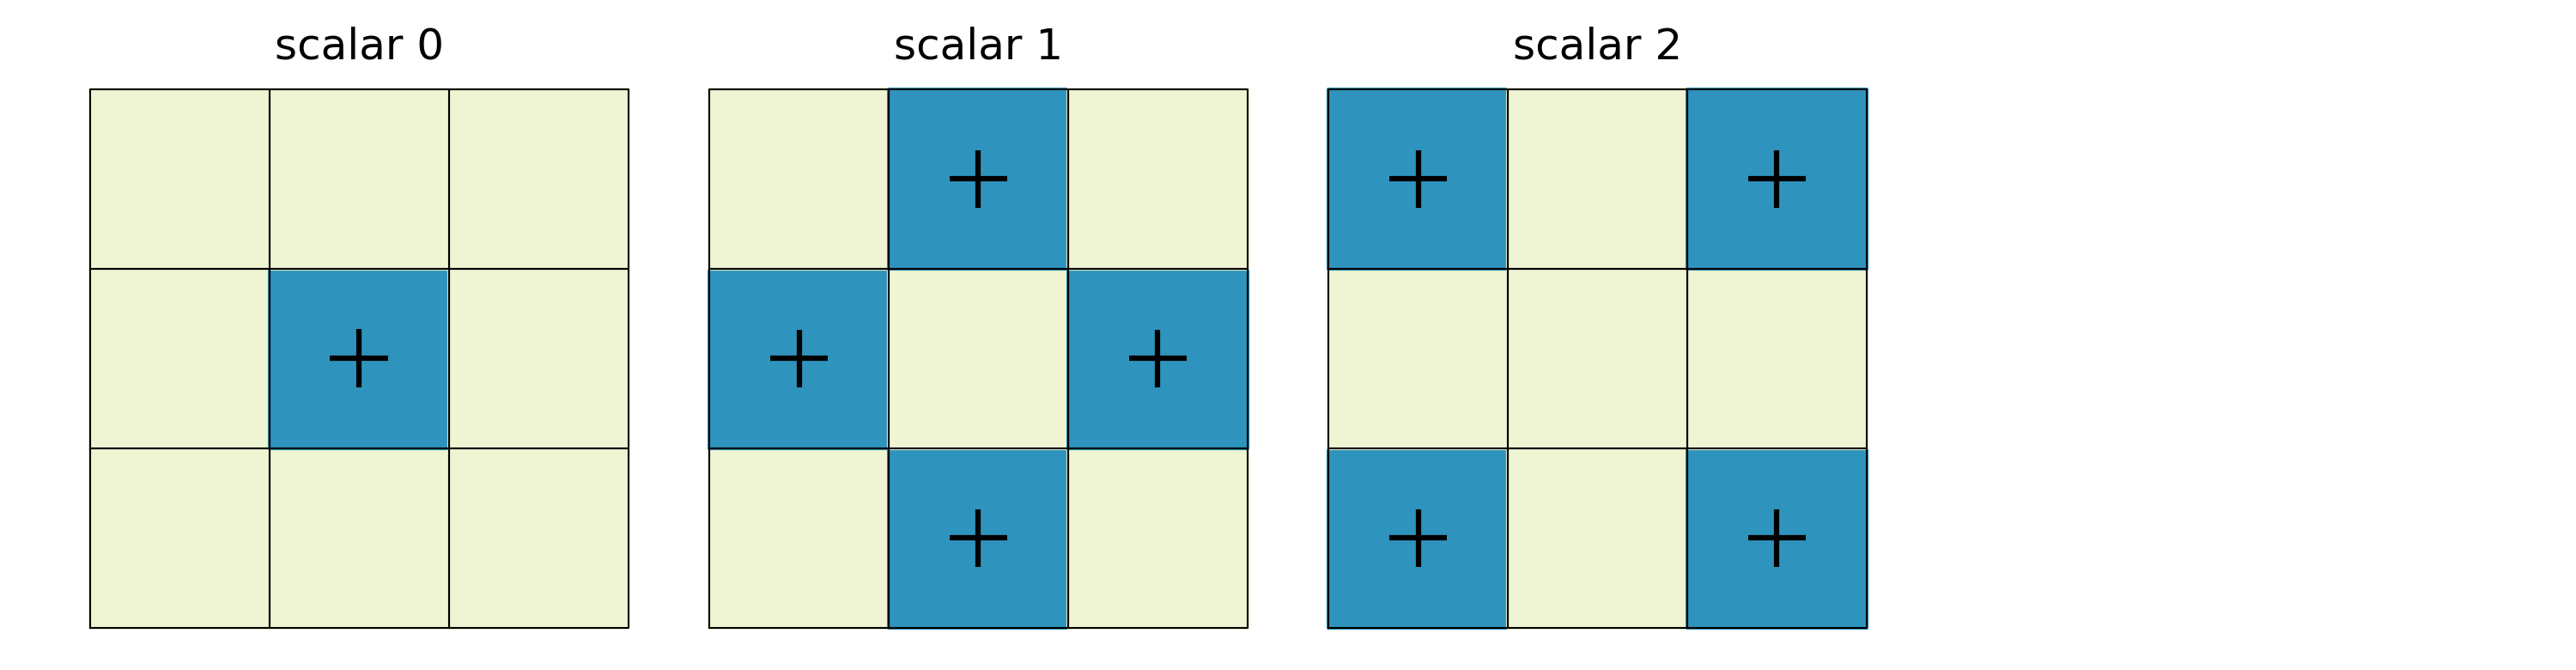
\includegraphics[width=\textwidth]{notebooks/filter+0_2_3.png}\\
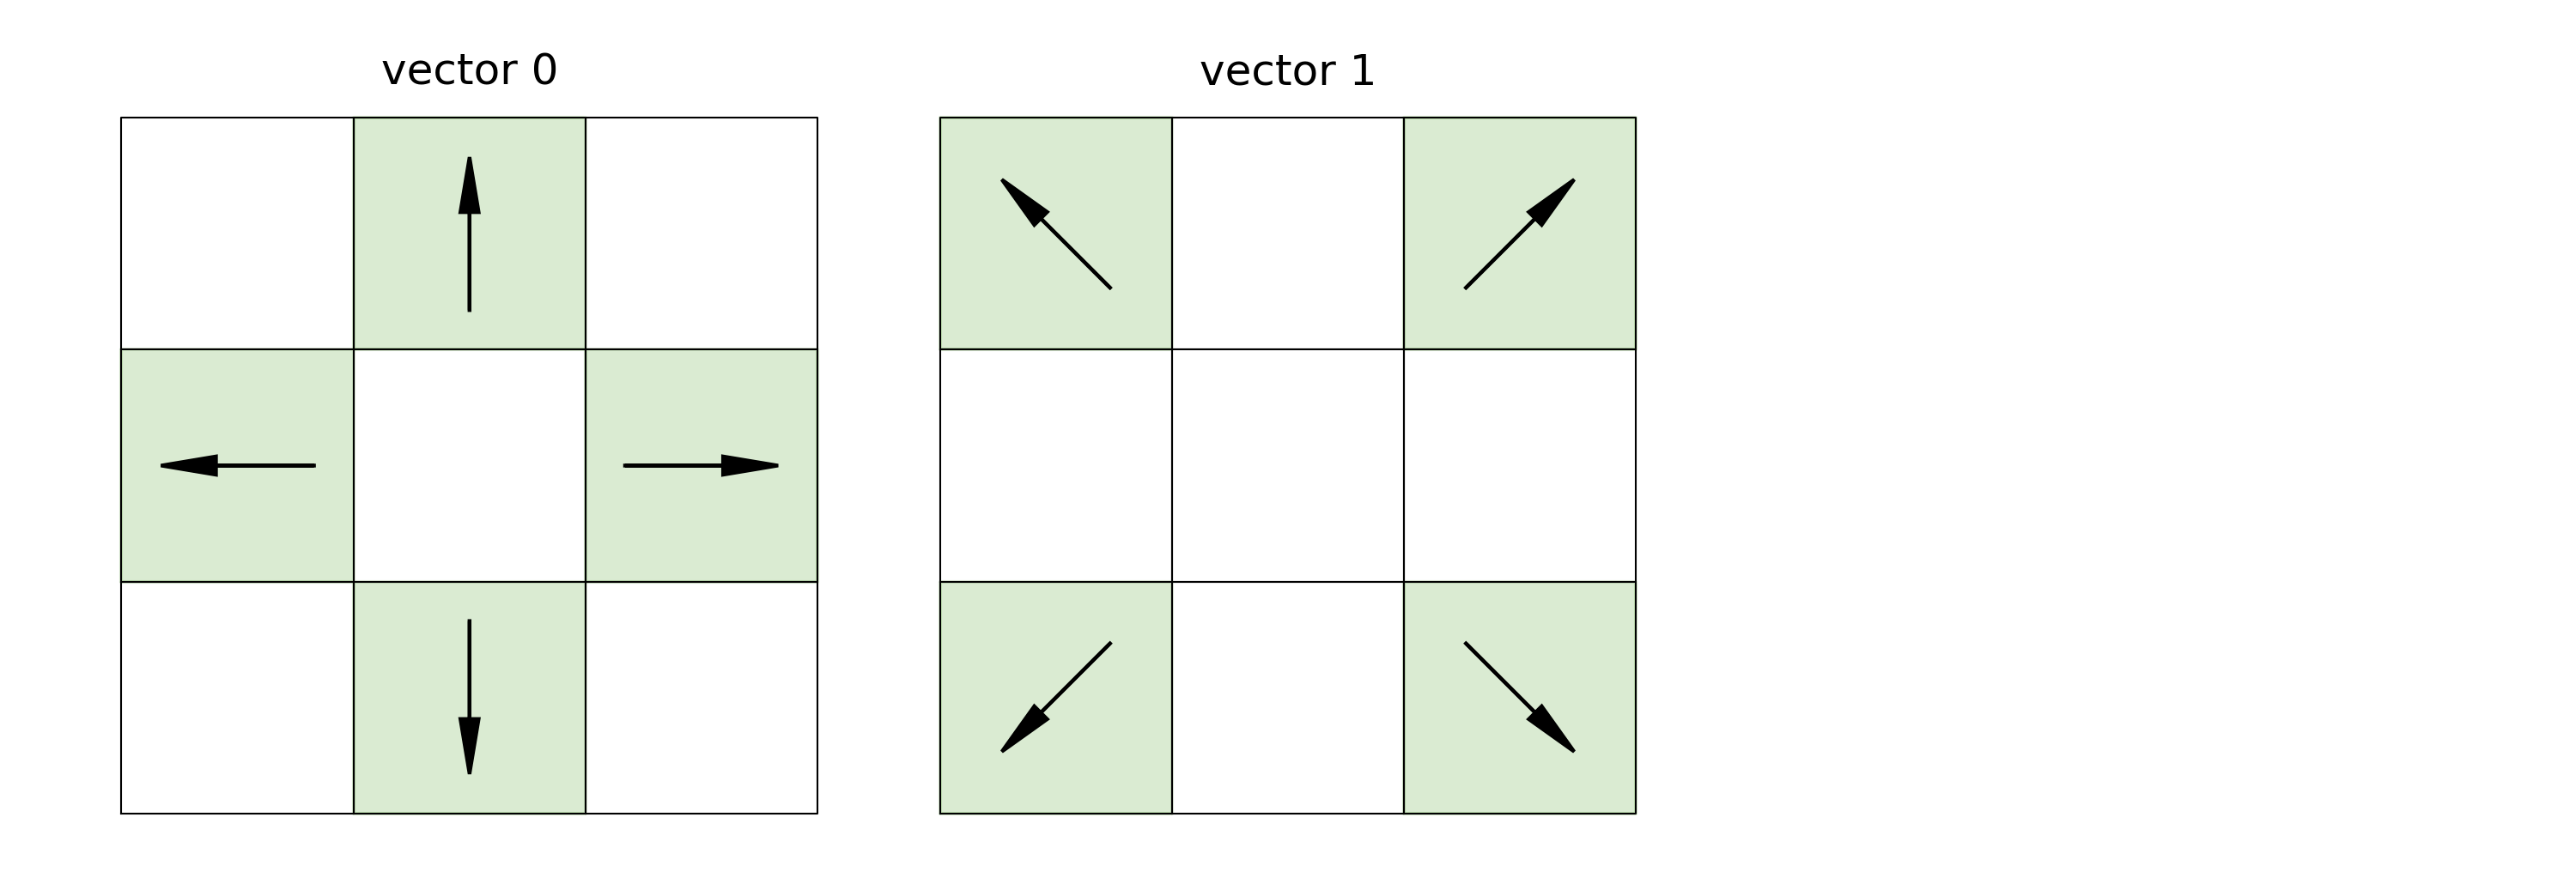
\includegraphics[width=\textwidth]{notebooks/filter+1_2_3.png}\\
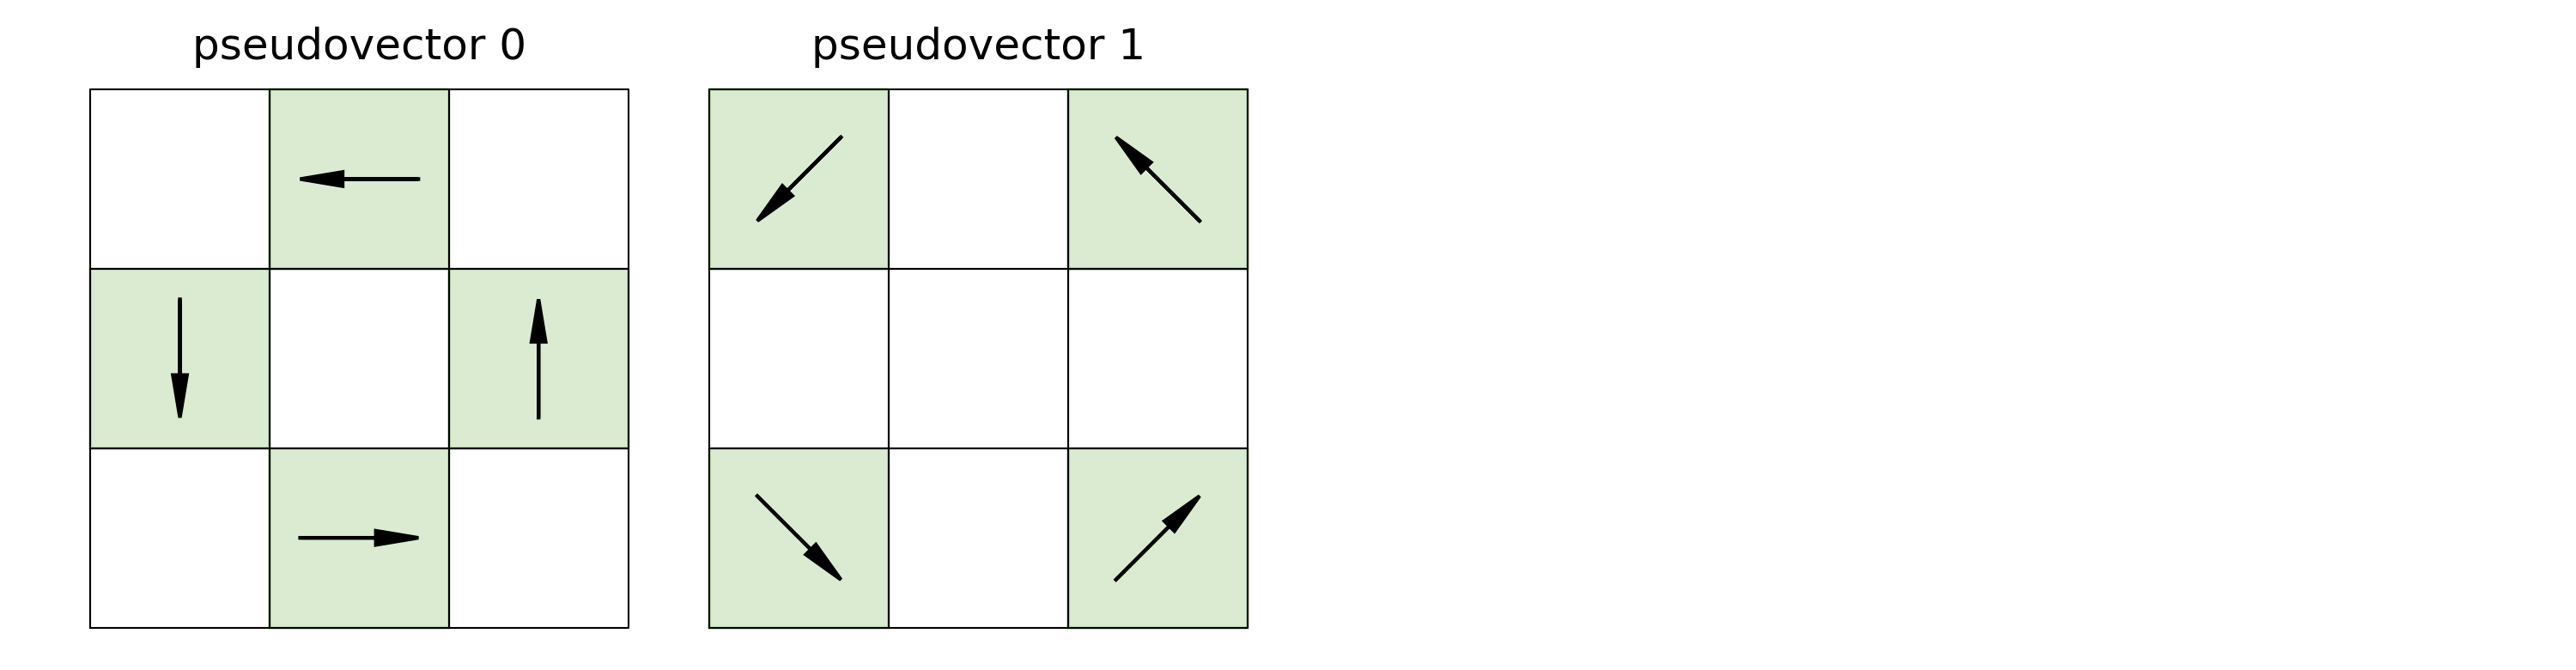
\includegraphics[width=\textwidth]{notebooks/filter-1_2_3.png}
\caption{All the filters for $d=2$, $m=1$. HOGG: notes!}
\end{figure}

\begin{figure}[tp]
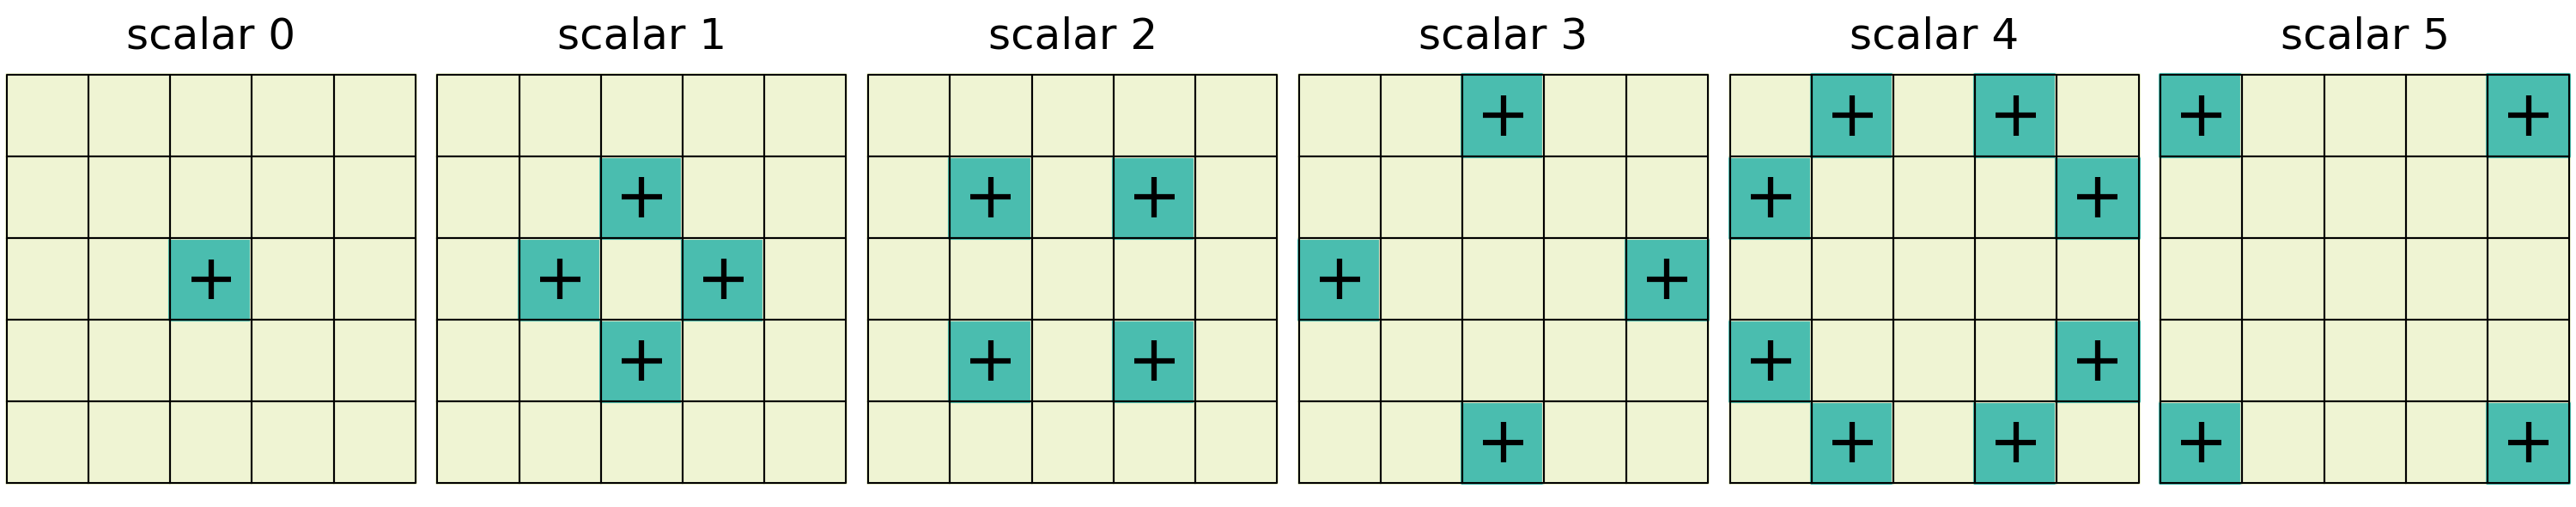
\includegraphics[width=\textwidth]{notebooks/filter+0_2_5.png}\\
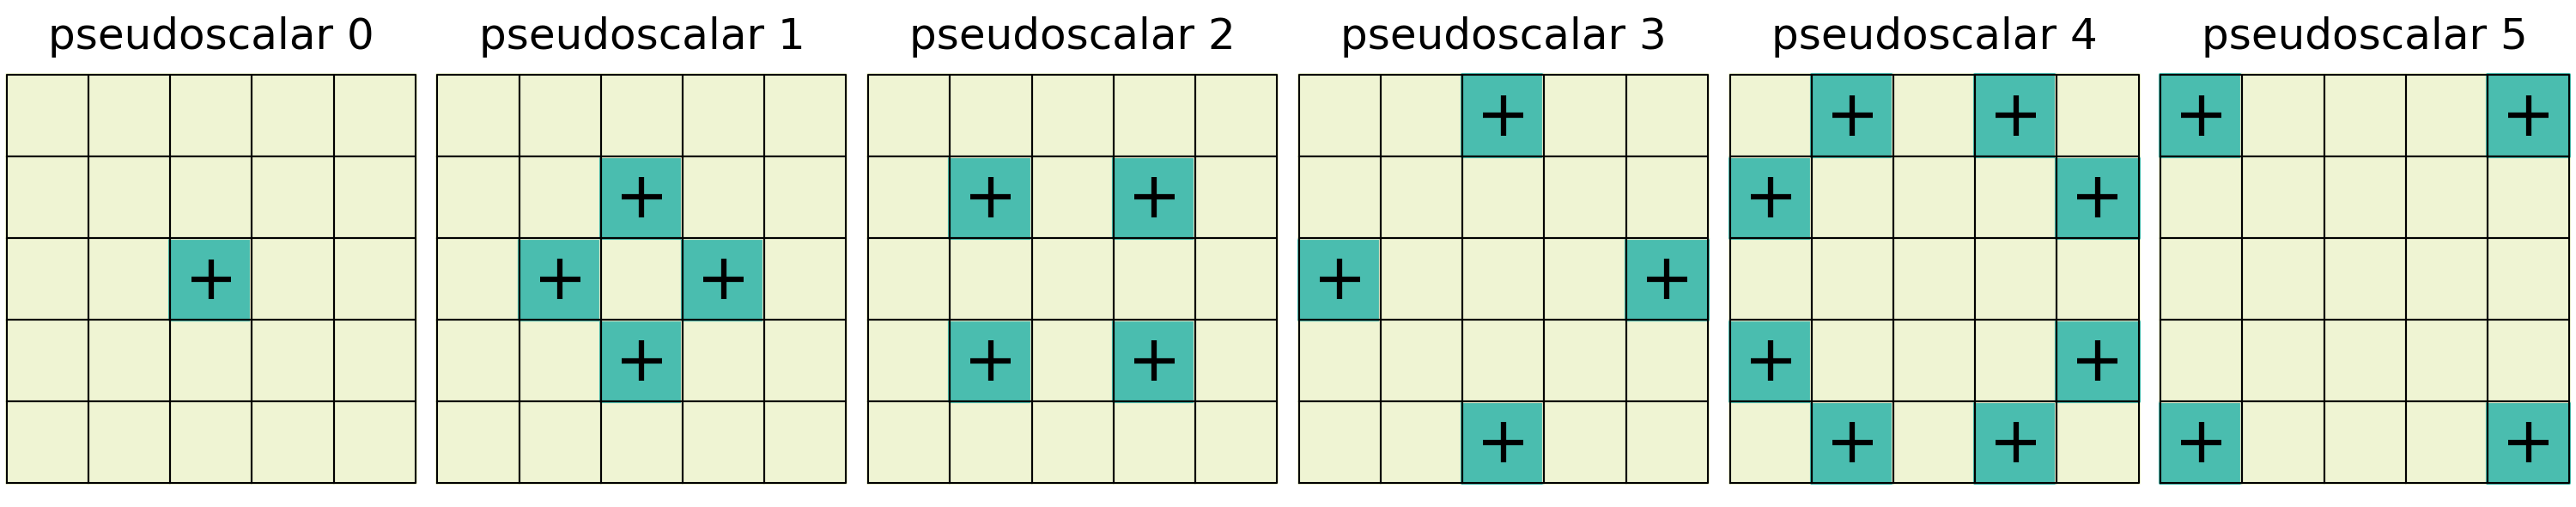
\includegraphics[width=\textwidth]{notebooks/filter-0_2_5.png}\\
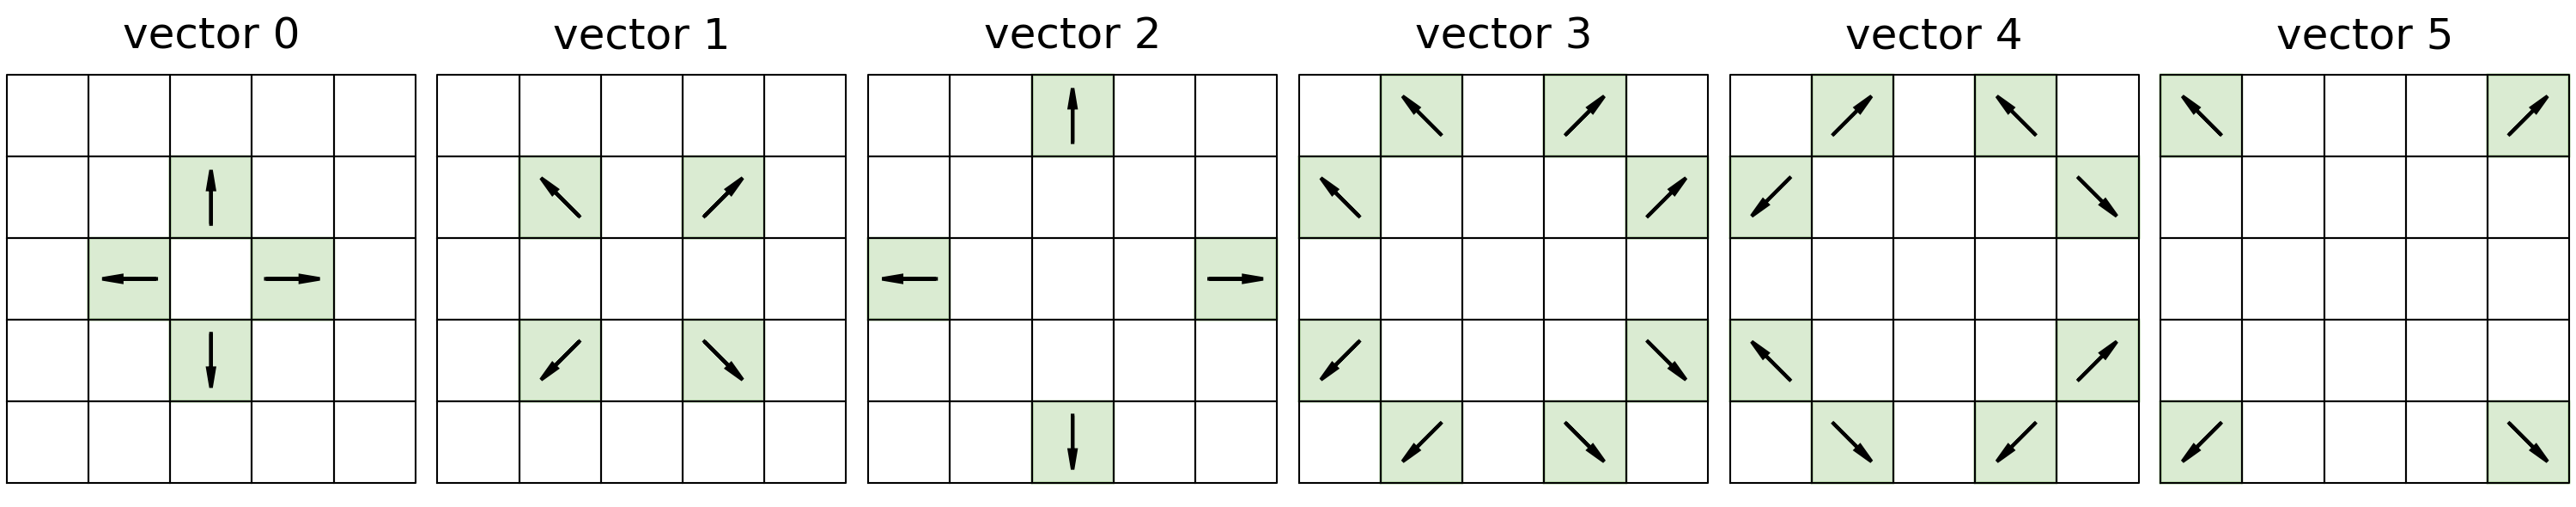
\includegraphics[width=\textwidth]{notebooks/filter+1_2_5.png}\\
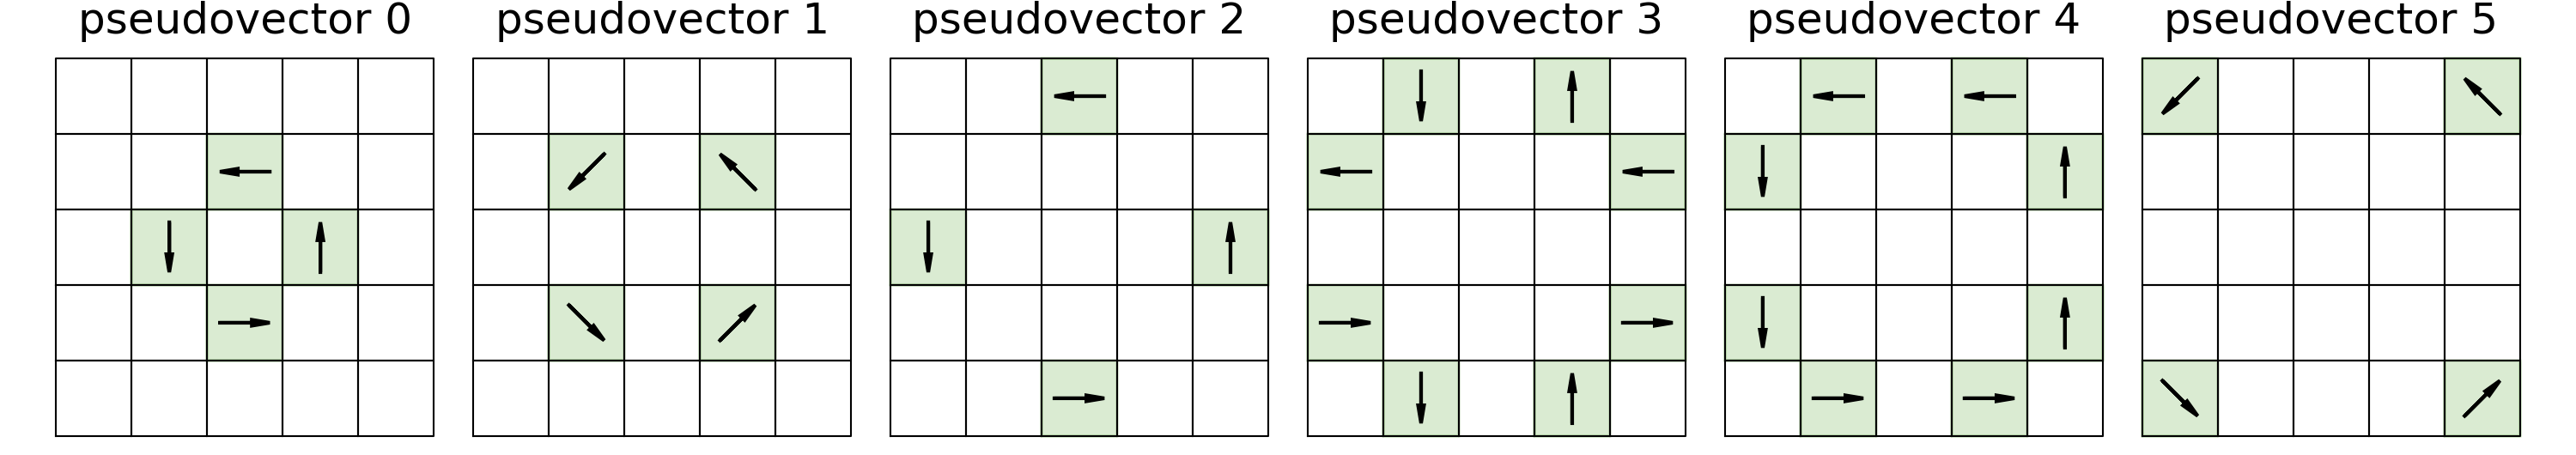
\includegraphics[width=\textwidth]{notebooks/filter-1_2_5.png}
\caption{All the filters for $d=2$, $m=2$. HOGG: notes!}
\end{figure}

Show all the filters for $d=2$, $M=5$.

Show all the filters for $d=3$, $M=3$.

Give a table saying how many filters there are for each $d$ and each $M$ at each $k$ and each parity.

Now show some fake-data geometric images and show the action of the $d=2$, $M=3$ filters on those images.

Now show contractions of products of the above on those images.

\section{Implementation notes}
\begin{itemize}
    \item find the invariant geometric filters
    \item geometric convolution operator
    \item pixel-wise outer product
    \item contraction operator, enumeration of all contractions
    \item output index permutation, enumeration of all permutations
    \item enumeration of all monomials up to a fix order and degree 
    \item remove repeated objects (SVD or just lstsq)?
    \item linear combinations 
    \item loss function
    \item optimization
\end{itemize}

\section{Discussion and comments}

Note that we never take eigenvalues. But these are also real scalars in some cases.

Note that pseudo-$k$-tensor filters only exist for certain triples of $(d, m, k)$.

\end{document}
